
%%%%%%%%%%%%%
%     FUTURE WORK    %
%%%%%%%%%%%%%

\begin{figure}
\centering
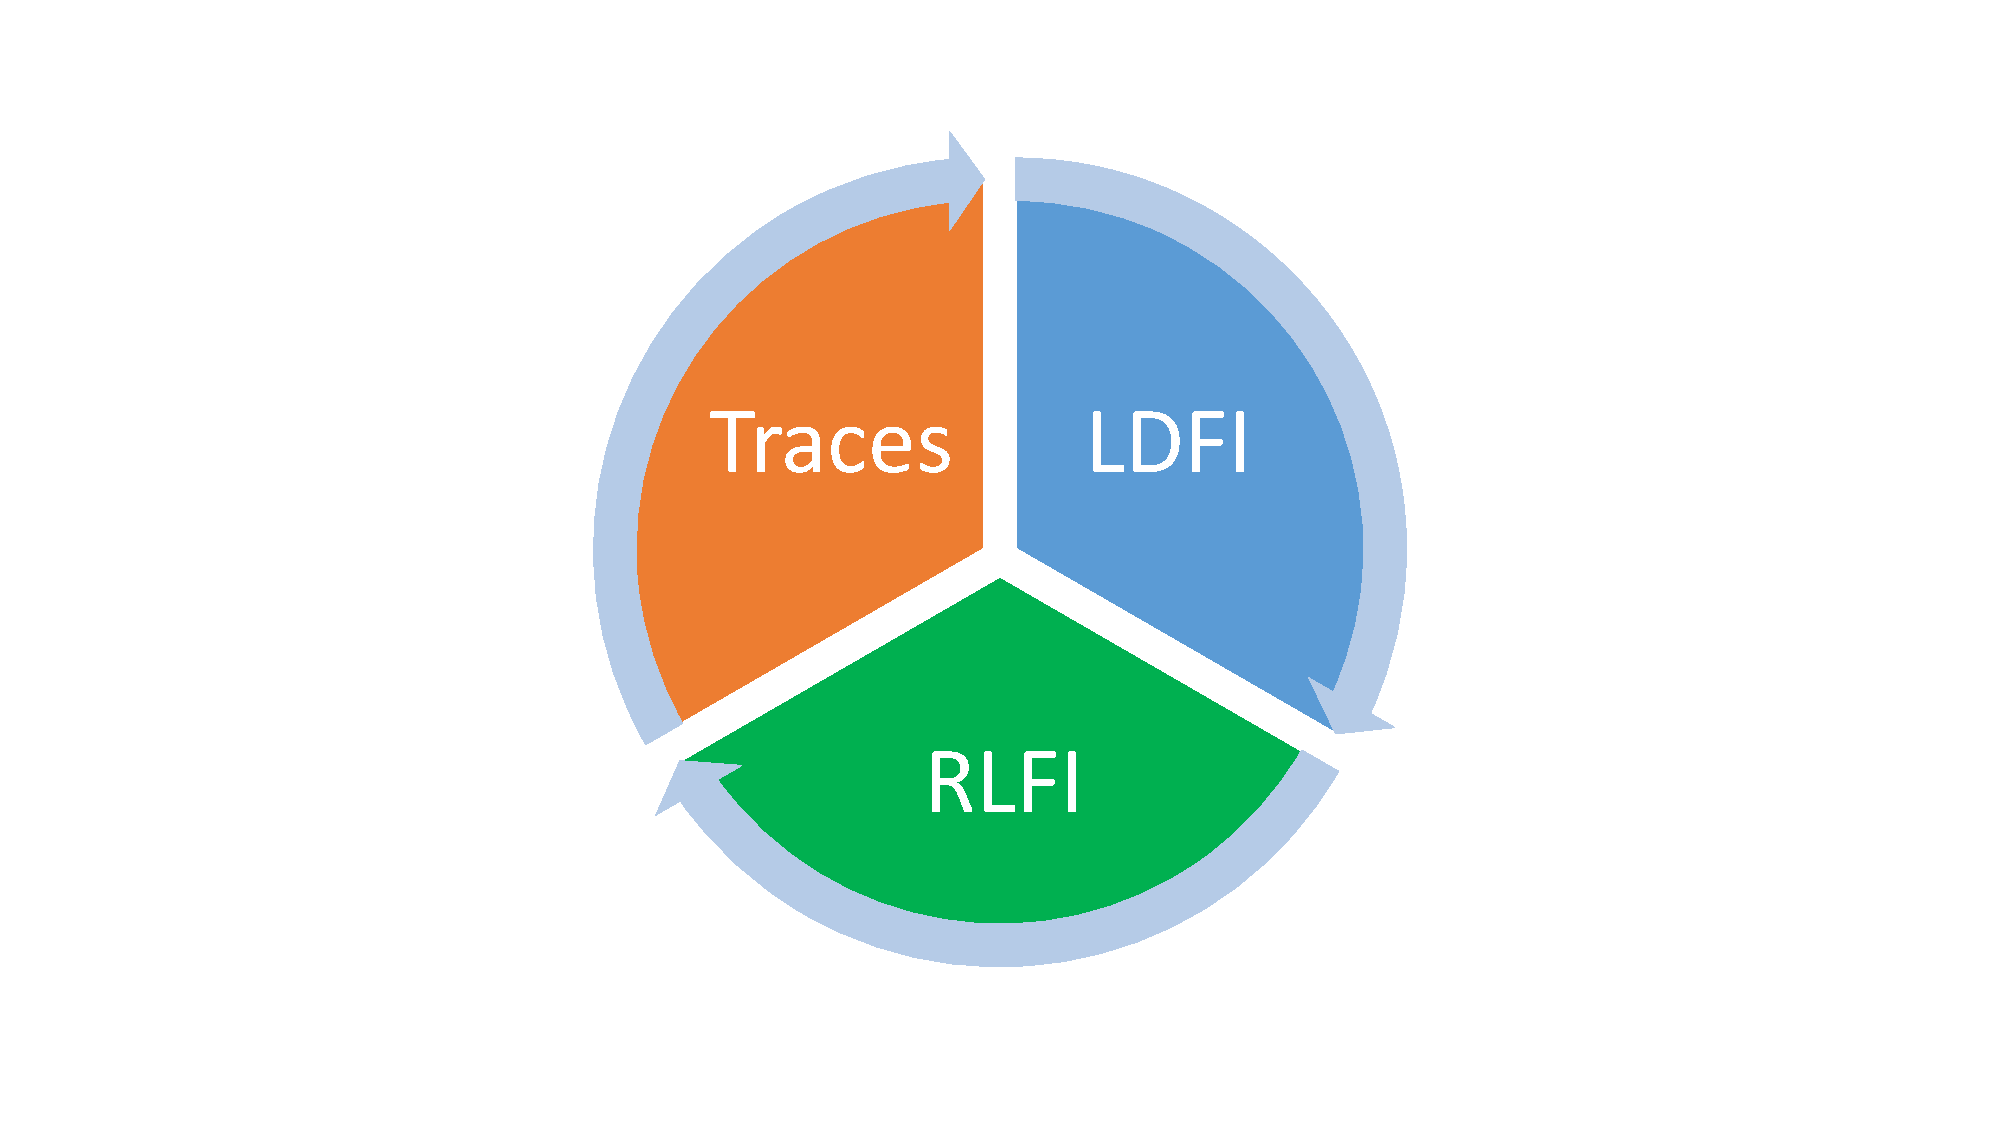
\includegraphics[width=8cm,height=10cm,keepaspectratio=true]{puzzle}
\caption{Fine-grained tracing, LDFI and RLFI completing the puzzle of debugging distributed systems}
\label{puzzle}
\end{figure}

\section{Future Work}
The current implementation of RLFI is but a proof-of-concept to show that we can perform fault injection experiments efficiently in a controlled setting, and obtain fine-grained traces to understand how the system reacts to such faults. Our current focus is to extend the implementation so that it supports a multitude of languages, not just Golang. While there is still much work to be done with RLFI, it is but one piece of a puzzle to understand and debug behavior of complex distributed systems, as shown in Figure\ref{puzzle}.

It is next to impossible to obtain a real life service from industry partners to perform our tests on, mainly because our partners do not want to risk their services being rendered useless or confidential information such as software architecture and personal client information to be exposed. Also, when compared to the real world, our toy architecture is but a measly branch in a huge tree of microservices. We hope to integrate our tracing and fault injection framework into a microservice generator which would generate graphs of size in resemblance of ones found in industry; this generator is undergoing development by a team member in our lab.

To manually dig through traces to find interesting points of failure for RLFI is a daunting task to say the least. Molly, an implementation of Lineage Driven Fault Injection, is a tool developed by Peter Alvaro et al.\cite{alvaro:ldfi} that is perfectly suited for our situation. We can feed the good traces that our system produces into LDFI, which will find the critical points of failure in our system. With the critical points found, we carefully inject the faults into the system and determine whether the fault handling mechanism of the service will is sufficient. We continue this cycle of tracing, reasoning, and injecting failure until we have a system that is robust enough for us to sleep soundly at night.

Currently the traces that results from our framework are cluttered and requires parsing to make it more human readable. We would like to develop a small, offline tool that will parse the traces into something that LDFI can understand and also produce a visual call graph for ease of verification. 

%%%%%%%
%    EOF     %
%%%%%%%